\documentclass[aspectratio=169]{beamer}

\usepackage[utf8]{inputenc}
%\usepackage{kotex}
\usepackage{tikz}
\usetikzlibrary{patterns}
\usepackage{xspace}

%\usepackage[sfdefault]{FiraSans}
%\usepackage{FiraMono}

% Plots
\usepackage{pgfplots}
\pgfplotsset{compat=1.14}
\usepgfplotslibrary{groupplots}
\usepgfplotslibrary{fillbetween}
\tikzset{mynode/.style={circle,draw,font=\small,minimum width=1cm,font=\sffamily}}
\pgfdeclarepatternformonly{north east lines wide}%
{\pgfqpoint{-1pt}{-1pt}}%
{\pgfqpoint{10pt}{10pt}}%
{\pgfqpoint{6pt}{6pt}}%
{
	\pgfsetlinewidth{0.1pt}
	\pgfpathmoveto{\pgfqpoint{0pt}{0pt}}
	\pgfpathlineto{\pgfqpoint{6.1pt}{6.1pt}}
	\pgfusepath{stroke}
}
\newcommand*{\FPR}{\operatorname{FPR}}
\newcommand*{\FNR}{\operatorname{FNR}}
\newcommand*{\FN}{\operatorname{FN}}
\newcommand*{\FP}{\operatorname{FP}}
\newcommand*{\EP}{\operatorname{EP}}

\newcommand*{\DUPLICATE}{\textsf{DUPLICATE}\xspace}
\newcommand*{\UNSEEN}{\textsf{UNSEEN}\xspace}

\usepackage{graphicx}


\usetheme{metropolis}           % Use metropolis theme


\titlegraphic{%
	\hfill\includegraphics[width=.3\textwidth]{logo-institute.png}\hfill
}


%\titlegraphic{\hfill \includegraphics[width=.2\textwidth]{logo-institute.png}\hfill}
\title{Approaching Optimal Duplicate Detection in a Sliding Window}
\date{August 30th, 2020}
\author{Rémi Géraud-Stewart, \textbf{Marius Lombard-Platet}, David Naccache}
\institute{Information security group, DIENS, École normale supérieure, PSL Research University (Paris, France)}

	

\begin{document}
\begin{frame}
	\maketitle
\end{frame}
\section{Introduction and motivation}

\begin{frame}{Finding duplicates}
	Let us consider a stream $E = (e_1, \dotsc, e_n, \dotsc)$ of elements, and a machine with a limited amount of memory $\mathcal M$.
	
	\begin{alertblock}{Question}
		How to detect if an element $e$ has already been seen in the past?
	\end{alertblock}%\pause

%	\begin{alertblock}{Second question}
%		Why do we care?
%	\end{alertblock}
%
%	\begin{exampleblock}{}
%			\begin{itemize}
%			\item Cache for CPU or webservers
%			\item Fraud detection (identical payments)
%			\item Cryptography (nonce reuse)
%			\item Security (check if URL is in a denylist)
%			\item ...
%		\end{itemize}
%	\end{exampleblock}

\end{frame}

\begin{frame}{Example}
This question leads to a second question: \pause

Why do we care?
\pause

There are several applications of detecting duplicates.
\begin{itemize}
	\item Cache for CPU or webservers
	\item Fraud detection (identical payments)
	\item Cryptography (nonce reuse)
	\item Security (check if URL is in a denylist)
	\item ...
\end{itemize}
\end{frame}

\begin{frame}{What is a duplicate filter?}
Quickly said, a duplicate filter is:
\begin{itemize}
	\item An algorithm operating with a finite amount of memory \pause
	\item When presented to a new element, outputs $\DUPLICATE$ or $\UNSEEN$ \pause
	\item Tries to keep memory of the previous elements
\end{itemize}
\end{frame}

\begin{frame}{Sub-problems of duplicate detection}
	In the literature, we can find several variants of the duplicate detection problem (DDP). We can match an element against:\pause
	\begin{itemize}
		\item a fixed, non-evolutive set (fixed duplicate detection, FDDP) \pause
		\item an evolutive set (streaming duplicate detection problem, SDDP) \pause comprising of:
		\begin{itemize}
			\item {\color<6->{red}the last $w$ elements of the stream ($w$DDP)} \pause
			\item all previous elements of the stream ($\infty$DDP)
		\end{itemize} 
	\end{itemize}
\pause
\end{frame}

\bgroup
\let\oldfootnoterule\footnoterule
\def\footnoterule{\only<2->\oldfootnoterule}
\begin{frame}{Prior work}
	Perfect solutions for $\infty$DDP and FDDP on an alphabet of size $\Gamma$ requires $\Gamma$ bits of memory\pause
	
	One can significantly reduce the amount of memory while keeping the errors under a certain value\footnote<2->{Burton H. Bloom. 1979. \textit{Space/Time Trade-offs in Hash Coding with Allowable Errors}} \pause
	
	Asymptotically, no filter can perform better than random on the $\infty$DDP\footnote<3->{Rémi Géraud, Marius Lombard-Platet, and David Naccache. 2019. \textit{Quotient hash tables: efficiently detecting duplicates in streaming data}}
	
\end{frame}

\begin{frame}{Contributions}
	We introduce a lower bound on the error rate for $\infty$DDP \pause
	
	We introduce two new structures for the $w$DDP:
	\begin{itemize}
		\item One for small values $w$
		\item One for adapting $\infty$DDP algorithms to the $w$DDP \pause
	\end{itemize}

	For these structures, we analyse their error rate and their resistance to adversarial attacks.
\end{frame}
\egroup


\section{Limitations of the $\infty$DDP}

\begin{frame}{Lower bound on $\infty$DDP error rate}
	Let be a filter of $M$ bits of memory on an alphabet of size $\Gamma$
	
	For $\FP_n, \FN_n$ the probability of a false positive/negative after $n$ insertions, and $\EP_n = \FN_n + \FP_n$ the error probability,\pause
	
	$$
	EP_n \geq 1 - \frac{1 - \left(1 - \frac{1}{|\Gamma|}\right)^{M}}{1 - \left(1 - \frac 1{|\Gamma|}\right)^n} 
	$$
	
	We observe that asymptotically, $\EP_\infty \gtrapprox 1 - \frac M\Gamma$
	
\end{frame}
\begin{frame}{Experimental saturation}
	Assuming a large alphabet of size $U$, a filter quickly saturates, to the point of answering randomly (FPR + FNR = 1)

	\begin{figure}
		\centering
		\scalebox{.7}{\begin{tikzpicture}
		%\begin{tikzpicture}
\begin{axis}[
	width=0.99\textwidth,
	xmode=log,
	xmin = 500,
	xmax = 200000000,
%	extra x ticks = {500},
	xlabel = {Size of the stream},
	ymax = 110,
    ymin = 0,
    ytick = {0, 20, ..., 120},
    ylabel = {$\FPR^\infty + \FNR^\infty (\times 100)$},
%    title = Artificial Stream,
	%legend pos = outer north east,
	legend style={at={(0.02,0.98)},anchor=north west,nodes={scale=0.9, transform shape}},%
    %width = 0.4\textwidth
]
%\nextgroupplot[
%xmode=log,
%xmin = 500,
%xmax = 350000000,
%%	extra x ticks = {500},
%xlabel = {Size of the stream},
%ymax = 110,
%ymin = 0,
%ytick = {0, 20, ..., 120},
%%    ylabel = {FPR + FNR},
%title = Uniform stream,
%    legend columns=1,
%    legend to name= legend_n,
%]
%% 1 QHT 
\addplot [color=red, mark=+] coordinates {
	(1000, 0)
	(10000, 0.28)
	(30000, 0.67)
	(50000, 5.55)
	(100000, 8.33)
	(300000, 24.07)
	(1000000, 56.52)
	(3000000, 81.41)
	(10000000, 93.74)
	(50000000, 98.83)
	(100000000, 99.03)
	(150000000, 99.21)
};
\addlegendentry{QHT}


%% 2 SQF
\addplot[color=blue, mark=x] coordinates {
	(1000, 0)
	(10000, 0.49)
	(30000, 1.38)
	(50000, 6.67)
	(100000, 10.4)
	(300000, 33.54)
	(1000000, 64.9)
	(3000000, 85.91)
	(10000000, 95.24)
	(50000000, 98.44)
	(100000000, 99.27)
	(150000000, 99.40)
};
\addlegendentry{SQF}

%% 3 Cuckoo
\addplot [color=teal, mark=triangle] coordinates {
	(1000, 0.2)
	(10000, 2.48)
	(30000, 6.63)
	(50000, 19.81)
	(100000, 28.8)
	(300000, 72.17)
	(1000000, 90.88)
	(3000000, 96.28)
	(10000000, 98.95)
	(50000000, 99.75)
	(100000000, 99.84)
	(150000000, 99.86)
};
\addlegendentry{Cuckoo}

%% 4 SBF 
\addplot [color=olive, mark=square, mark options = {scale=0.7}]coordinates {
	(1000, 0.3)
	(10000, 4.07)
	(30000, 10.18)
	(50000, 14.63)
	(100000, 46.64)
	(300000, 77.46)
	(1000000, 92.66)
	(3000000, 97.22)
	(10000000, 99.19)
	(50000000, 99.79)
	(100000000, 99.88)
	(150000000, 99.90)
};
\addlegendentry{SBF}

%%% 5 A2 
%\addplot [color=orange, mark=diamond]coordinates {
%	(1000, 0)
%	(10000, 0.03)
%	(30000, 0.38)
%	(50000, 1.1)
%	(100000, 3.92)
%	(300000, 19.6)
%	(1000000, 63.3)
%	(3000000, 86.66)
%	(10000000, 95.67)
%	(50000000, 98.94)
%	(100000000, 99.33)
%	(150000000, 99.46)
%};
%\addlegendentry{A2}
%
%
%% 5 bDBF 
%\addplot [color=magenta, mark=pentagon]coordinates {
%	(1000, 0)
%	(10000, 0.12)
%	(30000, 60.13)
%	(50000, 81.96)
%	(100000, 91.3)
%	(300000, 96.71)
%	(1000000, 98.94)
%	(3000000, 99.57)
%	(10000000, 99.87)
%	(50000000, 99.97)
%	(100000000, 99.98)
%	(150000000, 99.99)
%};
%\addlegendentry{b\_DBF}


\addplot[black, pattern=north east lines wide] coordinates
{
	(1000000, 0)
	(2000000, 49.63)
	(3000000, 66.16)
	(5000000, 79.40)
	(10000000, 89.31)
	(30000000, 95.90)
	(50000000, 97.18)
	(100000000, 98.09)
	(150000000, 98.34)
	(300000000, 98.50)
} \closedcycle; 

\end{axis}
%\end{tikzpicture}
		\end{tikzpicture}}
		\caption{Error rate (times 100) of DDFs of 1Mb as a function of stream length. Hatched area represents over-optimal (impossible) values.}
	\end{figure}
\end{frame}

\section{New Structures for the $w$DDP}

\begin{frame}{How to detect duplicates?}
	\textbf{Optimal detection}: $w\log_2 \Gamma$ bits.\pause
	
	\textbf{Initial idea}: all $w$ elements in a queue \pause
	\begin{itemize}
		\item optimal size, no error
		\item complexity increases with $w$
	\end{itemize}
\pause
	\textbf{Second idea}: add a counter for each element \pause
	\begin{itemize}
		\item O(1) complexity while keeping a constant size
		\item no errors
	\end{itemize}\pause

	Problem solved?
\end{frame}
\begin{frame}{Optimal detection}
	Let $\mathcal M$ the available memory, $w$ the size of the sliding window and $\Gamma$ the size of the alphabet, \pause
	
	\begin{itemize}
		\item If $M \geq w(\log_2(w) + 2\log_2(\Gamma))$ the wDDP can be perfectly solved in constant time. \pause
		
		\item If $M \geq 5w\log_2(w)$, the wDDP can be solved with an FPR of $\approx \frac 1w$, and FNR of $0$ and constant time.
	\end{itemize}

\end{frame}

\begin{frame}{Detection with smaller-than-optimal memory}
	As we just saw, detection is optimally solved when the memory is large enough. \pause
	
	So let's see what happens with smaller memory (or bigger $w$).
\end{frame}

\begin{frame}{A first try: SHF}
	We take the previous optimal solution: a queue and a counter \pause
	
	Rather than each element $e$, we store a \emph{hash} $h(e)$, of size $\lfloor \frac M{2w} - \frac 12 \log_2(w)\rfloor$. \pause 
	This value is chosen so that we can store a hash of each element of the sliding window.
	
	That's the SHF. \pause
	
	\begin{itemize}
		\item $\FN = 0$
		\item$\FP = 1 - \left(1 - \sqrt{w2^{-M/w}}\right)^w$
	\end{itemize}
\end{frame}

\begin{frame}{SHF saturation}

	\begin{columns}
		\begin{column}{0.5\textwidth}
	SHF saturates quickly after reaching a turning point.
	
	\vspace{6em}
	\textbf{Conclusion}: SHF can be used for optimal cases and a bit more.
		\end{column}
		\begin{column}{0.5\textwidth}  %%<--- here
			\begin{figure}[t]
			\centering
			\scalebox{.7}{
				\begin{tikzpicture}
\begin{semilogxaxis}[%legend pos = outer north east, 
	legend pos= north east,%
	xlabel=$w$, ylabel=$\FPR^w+\FNR^w (\times 100)$, xmin=40,ymin=0,mlineplot]

\addplot[color=blue, mark=o] table[x=w,y=Error] {graphs/shf.dat};

\addplot [draw=none,pattern=north west lines,pattern color=black,domain=10:1843,stack plots=y] {100} \closedcycle;
\addlegendentry{SHF}

%\addplot[color=red, mark=x] table[x=a,y=b] {graphs/CSHF.dat};
%\addlegendentry{CSHF}

\end{semilogxaxis}
\end{tikzpicture}

			}
			\caption{Error rate (times 100) of SHF on various $w$ sizes. Hatched area represents cases where optimal solutions exist.}
		\end{figure}
		\end{column}
	\end{columns}
\end{frame}

\begin{frame}{Another idea: Queuing Filter}
	The idea is to adopt $\infty$DDP filters into the $w$DDP context. For this, we create a queue of subfilters $\mathcal F_i$. \pause
	
	\begin{figure}
		\centering
		\scalebox{.8}{
			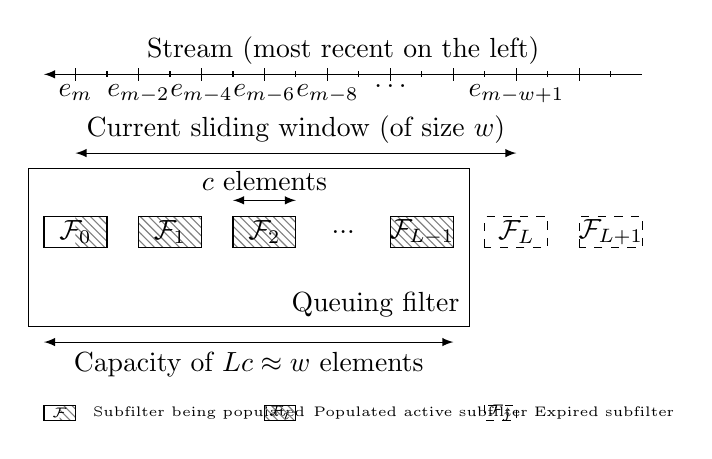
\begin{tikzpicture}[scale=0.4]
	
	% F_0 under construction
	\draw[pattern=north west lines, pattern color=gray, draw=none] (1, 0) rectangle (2, 1);
	\draw (0, 0) rectangle (2, 1) node[midway] {$\mathcal F_0$};

	
	% Other subfilters
	\draw[pattern=north west lines, pattern color=gray] (3, 0) rectangle (5, 1) node[midway] {$\mathcal F_1$};
	\draw[pattern=north west lines, pattern color=gray] (6, 0) rectangle (8, 1) node[midway] {$\mathcal F_2$};
	\node at (9.5, 0.5) {...};
	\draw[pattern=north west lines, pattern color=gray] (11, 0) rectangle (13, 1) node[midway] {$\mathcal F_{L-1}$};
	
	% old subfilters
	\draw[dashed] (14, 0) rectangle (16, 1) node[midway] {$\mathcal F_{L}$};
	\draw[dashed] (17, 0) rectangle (19, 1) node[midway] {$\mathcal F_{L+1}$};
	
	% arrows
	\draw [<->,>=latex] (6, 1.5) -- (8, 1.5) node[above, midway] {$c$ elements};
	\draw [<->,>=latex] (0, -3) -- (13, -3) node[below, midway] {Capacity of $Lc \approx w$ elements};
	\draw [<->,>=latex] (1, 3) -- (15, 3) node[above, midway] {Current sliding window (of size $w$)};
	
	%stream 
	\draw [<-, >=latex] (0, 5.5) -- (19, 5.5) node[above, midway] {Stream (most recent on the left)};
	\foreach \x in {1, 3,...,18}
	\draw (\x, 5.7) -- node[pos=0.5] (point\x) {} (\x, 5.3);
	
	\foreach \x in {2, 4,...,18}
	\draw (\x, 5.6) -- node[pos=0.5] (point\x) {} (\x, 5.4);

	\path (point1) node [below] {$e_m$};
	\foreach \x [evaluate=\x as \i using int(\x-1)] in {3, 5,..., 9}
	\path (point\x) node [below] {$e_{m-\i}$};
	\path (point11) node [below] {$\dots$};
	\path (point15) node [below] {$e_{m - w + 1}$};
	
	%queueing filter
	\draw (-0.5, 2.5) rectangle (13.5, -2.5) node[anchor=south east] {Queuing filter};
	
	% legend
	\draw[draw=none, pattern=north west lines, pattern color=gray] (0.5, -5) rectangle (1, -5.5);
	\draw (0, -5) rectangle (1, -5.5) node[midway] {\tiny $\mathcal F$};
	\draw (1.25, -5.25) node[anchor=west] {\tiny Subfilter being populated};
	
	\draw[pattern=north west lines, pattern color=gray] (7, -5) rectangle (8, -5.5) node[midway] {\tiny $\mathcal F_i$};
	\draw (8.25, -5.25) node[anchor=west] {\tiny Populated active subfilter};
	
	\draw[dashed] (14, -5) rectangle (15, -5.5) node[midway] {\tiny $\mathcal F_j$};
	\draw (1 5.25, -5.25) node[anchor=west] {\tiny Expired subfilter};
	\end{tikzpicture}
		}
	\end{figure}
\onslide<+->{We chose the parameters $L, c$ so that $Lc \approx w$.}
\end{frame}

\begin{frame}{Queueing Filter error probabilities}
	\begin{columns}
		\begin{column}{0.5\textwidth}
		FP and FN probabilities have been derived for a queueing filter using any kind of subfilter, but are a bit complicated to use. \pause
		
	\vspace{1em}
	
	Let's rather look at experiments.
		\end{column}
		\begin{column}{0.5\textwidth}  %%<--- here
			\begin{figure}[t]
			\centering
			\scalebox{.7}{
				\input{graphs/queue_bench.tex}
			}
			\caption{QHT-queuing filter and a QHT filter on various sliding window sizes. Hatched area represents values for which optimal solution exists.}
			\end{figure}
		\end{column}
	\end{columns}
\end{frame}

\section{Queueing Filter Security}
\begin{frame}{Filters in adversarial environment}
	An adversary chooses the stream sent to the filter \pause
	
	She does not have access to the memory state, only to the filter's output ($\DUPLICATE$ or $\UNSEEN$) \pause
	
	She wins the $(p, n)$-adversarial game if after a training period not longer than $n$, she can force a false positive (or a false negative) with probability $\geq p$
\end{frame}

\begin{frame}{FP security of queueing filter}
	Let $\mathcal Q$ be a queueing filter consisting of $L$ subfilters $\mathcal F_i$, each filled with $c$ items.
	
	If $\mathcal F$ is $(p, c)$-resistant to adversarial FP attacks and $cL \leq w$, then $\mathcal Q$ is $(1 - (1 - p)^L, w)$-resistant to FP attacks.
\end{frame}

\begin{frame}{FN security of queueing filter}
	Let $\mathcal Q$ be a queueing filter consisting of $L$ subfilters $\mathcal F_i$, each filled with $c$ items, and assume $w \leq (L-1)c$.
	
	Let $q = \displaystyle\min_{i \leq c} \FN_{\mathcal F, i}$, then $\mathcal Q$ is $(\min(1-q, p)^{L-1}p, w)$-resistant to adversarial FN attacks.
\end{frame}

\section{Conclusion}

\begin{frame}{Summing it up}
	\begin{itemize}
		\item For most cases, $\infty$DDP is an ill-posed problem and existing solutions are close to optimality \pause
		\item $w$DDP can be optimally solved if the memory is big enough \pause
		\item For w close (or inside) optimality, a excellent solution is the SHF \pause
		\item For $w$ slightly bigger, queueing filters are more interesting \pause
		\item For $w$ bigger, then existing $\infty$DDP solutions are the best solution
	\end{itemize}
\end{frame}

\begin{frame}[standout]{Thank you for your attention}
Any question?

\vspace{2em}

\footnotesize \texttt{remi.geraud@ens.fr\\marius.lombard-platet@ens.fr\\david.naccache@ens.fr}
\end{frame}

\end{document}